\documentclass[12pt]{article}
\usepackage{graphicx}
\graphicspath{ {../Results/} }

\title{Autocorrelation in weather}

\author{Amisha}

\date{23rd November, 2020}

\begin{document}
  \maketitle

  \section{Introduction}
    We investigated if temperatures of one year significantly correlated with the next year (successive years), across years in a given locationrom. Our temperature dataset was for Key West, Florida (1901-2000), with one value for every year.
  
  \section{Materials \& Methods}
  To answer the question we calculated the observed correlation between successive years and then 10000 correlations for randomly permuted year sequences.
  
  \section{Results}
  The preliminary data is shown in a scatterplot (Fig. 1). The observed correlation between successive years of temperature data has a value of 0.326. After calculating 10000 permutations of year sequences, we computed random correlation coefficients for them (Fig.2).
  \begin{figure}[h]
  \caption{Scatter plot of temperature data for Key West, Florida during the 20th century}
  \centering
  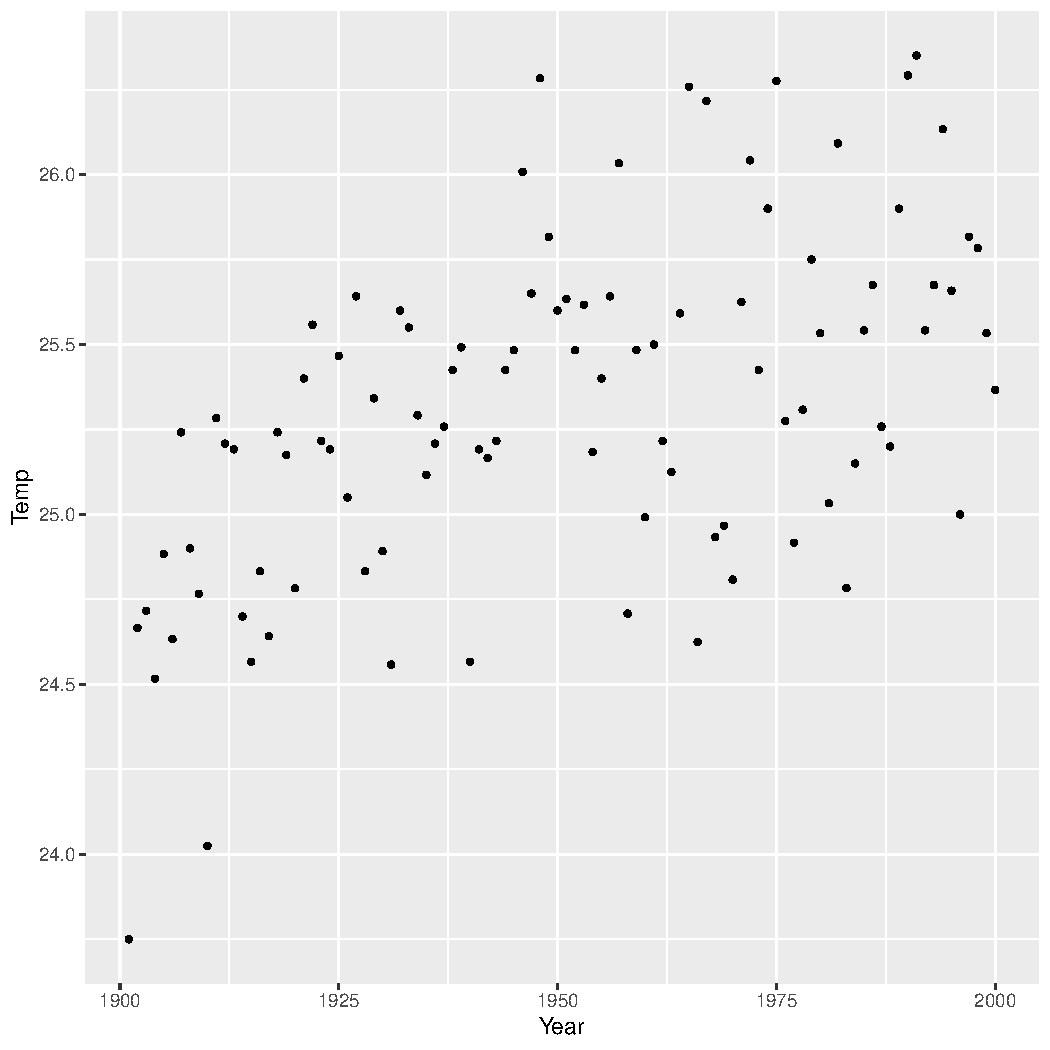
\includegraphics[scale=0.7]{ast_plot}
  \end{figure}
  \begin{figure}[h]
  \caption{Plot representing the distribution of correlation coefficients from randomly permuted temperature data for Key West, Florida during the 20th century. Blue vertical line represents observed correlation for original succession of years in the dataset.}
  \centering
  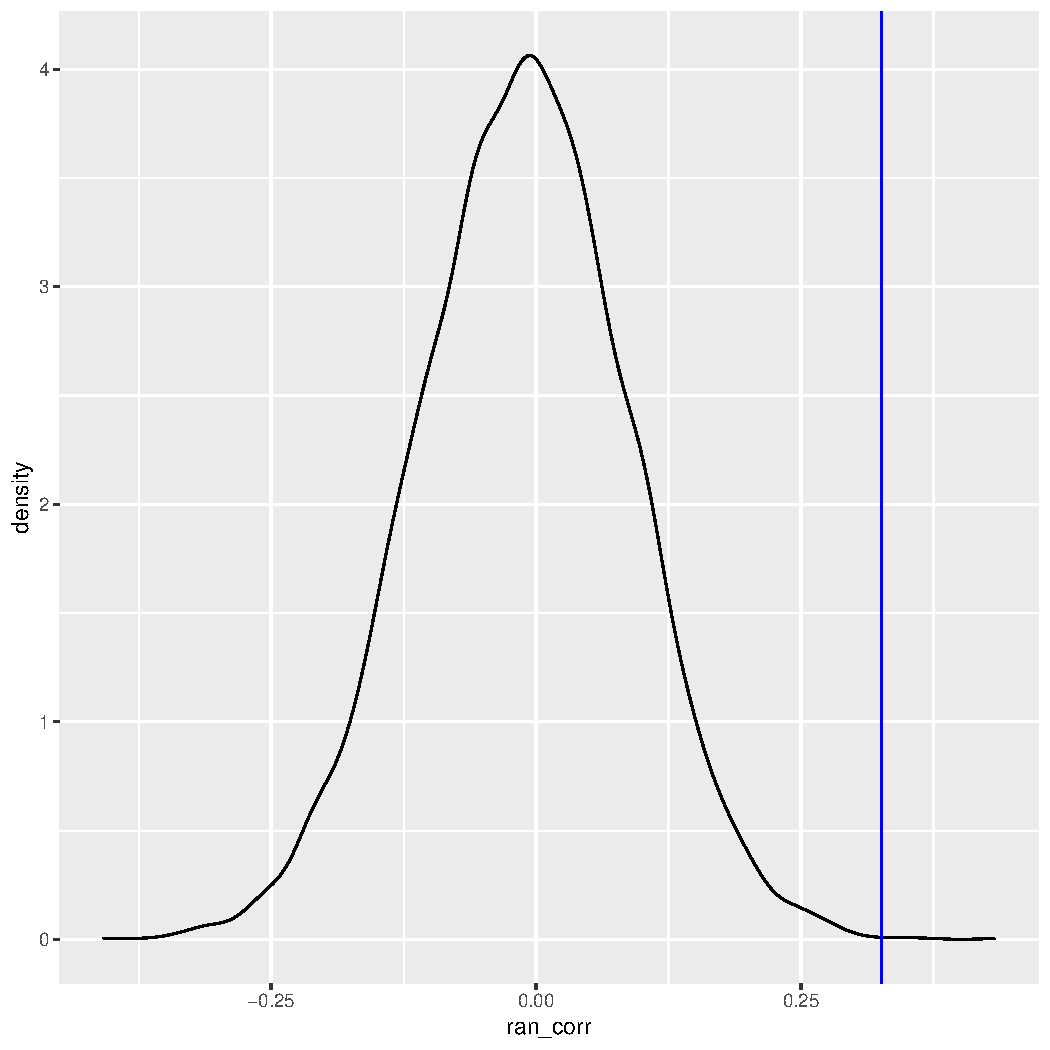
\includegraphics[scale=0.7]{ast_random_corr}
  \end{figure}
  
  
  To calculate an approximate p-value to determine whether the observed correlation is significantly different from the mean of the randomly correlated coefficients, we used this formula:

  \begin{equation}
    p-value = \frac{n.rancorr > obscorr}{iterations}
  \end{equation}

  We found the p-value to be 0.0003.

  \section{Discussion}
  The p-value indicates that the observed correlation between successive years is significantly different from that of randomly permuted sequences of years. This means that the temperature at any given year can be an adequate predictor of the average temperature in the next year.

\end{document}